\documentclass[12pt, a4paper]{article}
\usepackage[utf8]{inputenc}
\usepackage[T1]{fontenc}
\usepackage[slovene]{babel}
\usepackage{lmodern}
\usepackage{amsmath}
\usepackage{eurosym}
\usepackage{amsfonts}
\usepackage{hyperref}
\usepackage{tikz}


\usepackage{enumerate}
\setlength{\parindent}{0mm}

\newcommand{\novukaz}[2]{\underline {#1} \textit{#2}}

\newcounter{stevec}

\newenvironment{novookolje}[2]{\stepcounter{stevec} #1 #2 \thestevec}{}


\begin{document}
\begin{titlepage}
\begin{center}

\large
Univerza v Ljubljani\\
\normalsize
Fakulteta za matematiko in fiziko\\

\vspace{3 cm} 

\large
Eva Deželak in Ines Šilc\\

\vspace{0.5cm}
\LARGE
\textbf{KOCKARJEV PROPAD}

\vspace{0.5 cm}
\normalsize
Seminar

\vspace{1.5cm}
\normalsize
Mentor: doc. dr. Matija Vidmar

\vspace{3cm}


\vfill

\large Ljubljana, 2019

\end{center}
\end{titlepage}

\newpage

\tableofcontents
\vspace{20mm}
\newpage
 \section[Besedilo naloge]{Besedilo naloge}



Igralec $M$ ima $m$ enot denarja, igralec $N$ pa $n$ enot premoženja, $\{m,n\}\subset \mathbb{N}$. Zapored igrata igro na srečo v kateri ni neodločenih izidov; v vsaki igri dobi zmagovalec eno denarno enoto od poraženca; igralec $M$ zmaga vsakič z verjetnostjo $p\in (0,1)$, neodvisno od preteklosti. Igranje se konča, ko eden od igralcev bankrotira. Naj bo $T$ število iger, ki so potrebne, da eden od igralcev bankrotira. 
\begin{enumerate}[(i)]
\item Določi verjetnost, da bankrotira igralec $M$. Zakaj je  $T<\infty$ s.g.?
\item Predpostavi, da je $E[T]<\infty$ (za vsako izbiro $m$ in $n$). Določi $E[T]$. *Ali znaš utemeljiti, da je $E[T]<\infty$?
\end{enumerate}



\newpage

\section[Rešitev]{Rešitev}
\subsection{Računanje verjetnosti, da bankrotira igralec M}

Če je verjetnost, da zmaga igralec $M$, enaka $p$, potem je verjetnost, da zmaga igralec $N$, enaka $1-p$. Naj bo $A_a$ dogodek, da bankrotira igralec M, če začne z $a$ denarja, nasprotnik pa z $m + n - a$ denarja, kjer je $ a \in \{ 0, \dotso , m + n\}$. Za vsako število $a$, kjer je $ a \in \{ 0, \dotso , m + n\}$,  definiramo $p_a = P(A_a)$.
Poiskati želimo $p_m$, torej verjetnost, da propade igralec $M$, če ima $m$ denarja. 
\\

Naši hipotezi sta:
\\
$H$ - igralec M v prvem krogu zmaga (torej dobi 1 od igralca N)
\\
$H^C$ - igralec M v prvem krogu izgubi (torej da 1 igralcu N).
\\

Verjetnost, da igralec $M$ propade, če ima $a$ denarja je enaka:
\\
$$P(A_a) = P(A_a \vert  H) \cdot P(H) + P(A_a \vert  H^C) \cdot P(H^C),$$
 iz česar sledi, za $ a \in \{ 0, \dotso , m + n\}$,
\begin{equation*}
\begin{split}
p_a = p_{a+1} \cdot p + p_{a-1} \cdot (1 - p) &~ \Rightarrow \\
(p + 1 -p) \cdot p_a = p_{a+1} \cdot p + p_{a-1} \cdot (1 - p) &~ \Rightarrow \\
 p \cdot p_a + (1 - p) \cdot p_a = p_{a+1} \cdot p + p_{a-1} \cdot (1 - p) &~ \Rightarrow \\
p \cdot p_a - p_{a+1} \cdot p = (1 - p) \cdot  p_{a-1} - (1-p) \cdot p_a &~ \Rightarrow \\
p \cdot (p_a - p_{a+1}) = (1-p) \cdot (p_{a-1} - p_a). &~
\end{split}
\end{equation*}


Sedaj uvedemo novo oznako: $u_a = p_a - p_{a+1}$, za  $ a \in \{ 0, \dotso , m + n\}$. Torej velja tudi $u_{a-1} = p_{a-1} - p_a$, zato sledi, da je:
$$p \cdot u_a = (1 - p) \cdot u_{a-1}.$$
Torej: $$u_a = \frac{1-p}{p} \cdot u_{a-1}.$$

Če sedaj uvedemo še oznako $r:=\frac{1-p}{p}$, dobimo:
$$u_a = r \cdot u_{a-1}.$$


Od tod lahko izrazimo vse člene z začetnim (torej z $u_0$):
$$u_1 = r \cdot u_0$$
$$u_2 = r \cdot u_1 = r \cdot r \cdot u_0 = r^2 \cdot u_0$$ 
$$\cdots $$
$$u_a = r^a \cdot u_0$$ za $ a \in \{ 0, \dotso , m + n\}.$

Vemo, da če ima eden od igralcev ves denar, potem gotovo zmaga, če pa ga nima nič, potem gotovo izgubi, zato je:
$$p_c = 0 \textrm{, kjer je } c := m + n \textrm{ in } p_0 = 1.$$

Sedaj lahko najprej $u_0$ izrazimo z začetnimi podatki \footnote{Razen, ko je $r = 1$, glej poseben primer \ref{Poseben primer za r = 1}} :
\begin{equation*}
\begin{split}
1 = p_0 - p_c &= (p_0 - p_1) + (p_1 - p_2) + \cdots + (p_{c-1} - p_c) = \\
        &= u_0 + u_1 + u_2 + \cdots + u_{c-1} = \\
        &= u_0 + r \cdot u_0 + r^2 \cdot u_0 + \cdots + r^{c-1} \cdot u_0 = \\
        &= u_0 \cdot (1 + r + r^2 + \cdots + r^{c-1}) = \\
        &= u_o \cdot \frac{r^c - 1}{r-1}  
\end{split}
\end{equation*}  

Iz tega sledi: $$u_0 = \frac{r-1}{r^c -1}.$$


Sedaj lahko izračunamo verjetnost za propad prvega igralca (vemo, da je $u_m = p_m - p_{m+1}$):
\begin{equation*}
\begin{split}
p_m &= u_m + p_{m+1} = u_m + u_{m+1} + p_{m+2} = \\
    &= u_m + u_{m+1} + u_{m+2} + u_{m+3} + \cdots + u_{m+n-1} + p_{m+n} = \\
    &= u_m + u_m \cdot r + u_m \cdot r^2 + \cdots + u_m \cdot r^{n-1} + 0 = \\
    &= u_m + u_m \cdot \frac{1-p}{p} + u_m \cdot (\frac{1-p}{p})^2 + u_m \cdot (\frac{1-p}{p})^3 + \cdots + u_m \cdot (\frac{1-p}{p})^{n-1} = \\
    &= u_m \cdot (1 + \frac{1-p}{p} + (\frac{1-p}{p})^2 + \cdots + (\frac{1-p}{p})^{n-1}) 
    = u_m \cdot \frac{(\frac{1-p}{p})^n - 1}{\frac{1-p}{p} - 1} = \\
    &= r^m \cdot u_0 \cdot \frac{(\frac{1-p}{p})^n - 1}{\frac{1-p}{p} - 1}  
    = (\frac{1-p}{p})^m \cdot \frac{\frac{1-p}{p} - 1}{(\frac{1-p}{p})^{m+n} -1}\cdot \frac{(\frac{1-p}{p})^n - 1}{\frac{1-p}{p} - 1} = \\
    &= \frac{(\frac{1-p}{p})^n - 1}{(\frac{1-p}{p})^{m+n} -1} \cdot (\frac{1-p}{p})^m 
    = \frac{(\frac{1-p}{p})^{m+n} - (\frac{1-p}{p})^m}{(\frac{1-p}{p})^{m+n} -1} = \\
    &= \frac{\frac{(1-p)^{n+m}}{p^n} - (1-p)^m}{\frac{(1-p)^{n+m}}{p^n} - p^m} = 
    \frac{(1-p)^{n+m} - (1-p)^m \cdot p^n}{(1-p)^{m+n} - p^{m+n}}.
\end{split} 
\end{equation*}
Torej, dobili smo verjetnost za propad igralca $M$.

Da se bo igra skoraj gotovo končala, mora biti vsota verjetnosti, da bankrotira igralec $M$, in da bankrotira igralec $N$, enaka $1$:
\begin{equation*}
\begin{split}
&~\frac{(1-p)^{m+n}-p^m (1-p)^n}{(1-p)^{m+n}-p^{m+n}}+\frac{p^{m+n}-p^m
   (1-p)^n}{p^{m+n}-(1-p)^{m+n}} =\\
= &~\frac{(1-p)^{m+n}-p^m (1-p)^n}{(1-p)^{m+n}-p^{m+n}}-\frac{p^{m+n}-p^m
   (1-p)^n}{(1-p)^{m+n}-p^{m+n}} =\\
= &~\frac{(1-p)^{m+n}-p^m (1-p)^n-p^{m+n}+p^m
   (1-p)^n}{(1-p)^{m+n}-p^{m+n}} =\\
= &~\frac{(1-p)^{m+n}-p^{m+n}}{(1-p)^{m+n}-p^{m+n}} \\
= &~1.
\end{split} 
\end{equation*}


\subsubsection{Poseben primer}
\label{Poseben primer za  r = 1}
Vprašanje se pojavi, kaj se zgodi, če imata oba igralca enako verjetnost za zmago, torej $p = 1 - p = \frac{1}{2}$. Takrat namreč zgornji izračun ni mogoč, saj bi prišlo do deljenja z $0$. Iz tega dobimo, da je 
$$r = \frac{1 - \frac{1}{2}}{\frac{1}{2}} = 1.$$

V tem primeru so $u_0, u_1, \dotso, u_n$ med seboj enaki, torej:
$$u_k = r^k \cdot u_0 = u_0.$$

Posledično še lažje izrazimo $u_0$, na način:
$1 = c\cdot u_0$, torej $u_0 = \frac{1}{c}.$

V tem primeru je naša iskana verjetnost za igralca $M$ enaka
\begin{equation*}
\begin{split}
p_m &= u_0 \cdot (c - m) = \frac{c-m}{c} = \\
		&= \frac{m + n - m}{m + n} = \frac{n}{m + n}.
\end{split} 
\end{equation*}

Ponovno mora veljati, da je vsota verjetnosti, da bankrotira igralec $M$, in da bankrotira igralec $N$, enaka $1$, je pa izračun v tem primeru veliko krajši. Torej: 
$$\frac{n}{m + n} + \frac{m}{m + n} = \frac{n + m}{m+ n} = 1.$$


\subsection{Računanje $E[T]$}
\subsubsection{Predpostavka, da je $E[T] < \infty$}
Razmislimo najprej, zakaj je $E[T] <\infty$. Če lahko čas $T$, ko se igra konča, navzgor omejimo s časom $\widetilde{T}$, katerega upanje lahko lažje izračunamo, in dokažemo, da je končno, bo sledilo, da je tudi $E[T]$ končna. Vsakič, ko vidimo $m+n-1$ zaporednih dobitkov igralca M, se je igra gotovo končala, saj je v najslabšem primeru začel z 1 enoto denarja in je blo potrebnih $m+n-1$ iger, da se je tekma zaključila.\\

Definirajmo: 
\[
X_n := \left\{
\begin{array}{rl}
1; & \textrm{če zmaga igralec M}\\
0; & \textrm{če zmaga igralec N}
\end{array}
\right.
\]

Tako lahko navzgor ocenimo $T$:
$$T \leq inf\{ l \in \mathbb{N}: \textrm{v zaporedju } X_1, \dots, X_l \textrm{ smo videli } m+n \textrm{ zaporednih enic} \leq$$ 
$$
\begin{array} {lll} 
\leq (m+n)\cdot inf\{ l \in \mathbb{N}:& X_1, \dots, X_{m+n}; & \textrm{vsebuje same enice, ali} \\ 
&X_{m+n+1}, \dots, X_{2(m+n)};& \textrm{vsebuje same enice, ali}\\
&\dots \\
&X_{(l-1)(m+n)+1}, \dots, X_{l(m+n)}; & \textrm{vsebuje same enice}\}=
\end{array}$$
$~~= (m+n)\cdot G_l =: \widetilde{T}$\\

Časovno os razdelimo na intervale dolžine $m+n$, znotraj katerih čakamo, da zaporedje $\{X_l\}_{l \in \mathbb{N}}$ vsebuje same enice:
\begin{center}
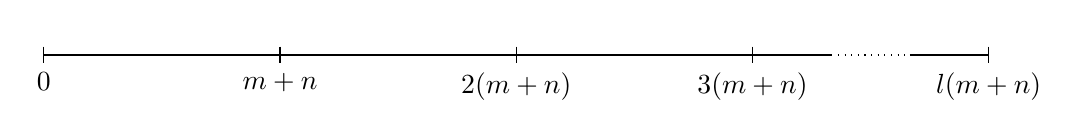
\begin{tikzpicture}

    \draw (0,0) -- (10,0);
	\draw[dotted] (10,0) -- (11,0);
	\draw (11, 0) -- (12, 0);
 
    \foreach \x in {0,3,6,9,12}
      \draw (\x cm,3pt) -- (\x cm,-3pt);

    \draw (0,0) node[below=3pt] {$ 0 $} node[above=3pt] {$   $};
    \draw (3,0) node[below=3pt] {$m+n$} node[above=3pt] {$  $};
    \draw (6,0) node[below=3pt] {$2(m+n)$} node[above=3pt] {$  $};
    \draw (9,0) node[below=3pt] {$3(m+n)$} node[above=3pt] {$ $};
	\draw (12,0) node[below=3pt] {$l(m+n)$} node[above=3pt] {$ $};
\end{tikzpicture}
\end{center}

Vsako zaporedje $\{X_l\}_{l \in \mathbb{N}}$ v $\widetilde{T}$ je zaporedje Bernoullijevih spremenljivk, saj pri upanju računamo verjetnost, da se v $m+n$ ponovitvah dogodek zgodi natanko $m+n$-krat. Torej $X_l$\textasciitilde $Ber(p^{m+n})$, medtem ko je zaporedje 
$\{X_l\}_{l \in \mathbb{N}}$ porazdeljeno geometrijsko, torej $G_l$\textasciitilde $Geom(p^{m+n})$, saj čakamo, da se dogodek, ko zaporedje vsebuje same enice, zgodi natanko enkrat. Sledi:

$$E[G_l]=\frac{1}{p^{(m+n)}} \Longrightarrow E[\widetilde{T}] = \frac{m+n}{p^{(m+n)}} < \infty$$

\newpage
\subsubsection{Računanje $E[T]$ za vsak $m$ in $n$}
Za dejanski izračun matematičnega upanja števila iger rešujemo enačbo oblike: $$E[T|M=x] = p\cdot E[T|M=x+1] + (1-p)\cdot E[T|M=x-1] + 1,$$ kjer je prvotno premoženje igralca M enako x, kar zaradi lažjega zapisa prevedemo na obliko $f(x) = p\cdot f(x+1) + (1-p) \cdot f(x-1) + 1 ~ \textrm{oziroma} $ 
\begin{equation}
\label{prvotna rekurzivna}
p\cdot f(x+2) - f(x+1) + (1-p)\cdot f(x) = -1,
\end{equation}
kjer je $f(x):=E[T|M=x]$ in $x \in \mathbb{N}$. Tu smo predpostavili, da je $E[T] < \infty$, da lahko enolično zadostimo rekurzivni enačbi. 
Rešujemo torej nehomogeno rekurzivno enačbo \footnote{Razen, ko je $p=\frac{1}{2}$, glej poseben primer \ref{Poseben primer za 1/2} } , katere rešitev je vsota homogene in ene partikularne rešitve. \\

Rešimo najprej homogeni del. Rešujemo enačbo: 
\begin{equation}
\label{homogena}
p\cdot f(x+2) - f(x+1) + (1-p)\cdot f(x) = 0.
\end{equation}
S pomočjo karakterističnega polinoma dobimo enačbo: $$p\cdot  \lambda ^2 - \lambda + (1-p) = 0$$ $$\lambda _{1, 2}= \frac{1 \pm \sqrt{1 - 4p(1-p)}}{2p} = \frac{1 \pm (2p-1)}{2p}.$$
Dobimo $\lambda _{1} = 1$ in $\lambda _{2} = \frac{1-p}{p}$. Rešitev enačbe (\ref{homogena}) je oblike $A\cdot 1^x + B(\frac{1-p}{p})^x$, oziroma: $$A+ B \bigg( \frac{1-p}{p} \bigg )^x. $$

Partikularno rešitev iščemo z nastavkom $f(x)= Cx1^x$ oziroma $f(x)= Cx$. Vstavimo v enačbo (\ref{prvotna rekurzivna}) in dobimo: 
\begin{equation*}
\begin{split}
 &~pC(x+2)-C(x+1)+(1-p)Cx=-1\\
\Leftarrow & ~Cpx+2Cp-Cx-C+Cx-Cpx=-1 \\
\Leftarrow & ~C(2p-1)=-1\\
\Leftarrow & ~C=\frac{-1}{2p-1} = \frac{1}{1-2p}.\\
\end{split}
\end{equation*}
 
Partikularna rešitev je: $$f(x)=\frac{x}{1-2p}.$$

Splošna rešitev\footnote{Razen, ko je $p=\frac{1}{2}$, glej poseben primer \ref{Poseben primer za 1/2} } enačbe (\ref{prvotna rekurzivna}) je: $$A + B\bigg( \frac{1-p}{p} \bigg )^x+\frac{x}{1-2p}.$$

Upoštevamo lahko še robna pogoja:
\begin{enumerate}
\item Pričakovano število iger, če smo brez denarja, je 0, saj se takrat igra konča. Pogoj zapišemo v obliki $E[T|M= 0] = f(0) = 0$. Vstavimo v splošno rešitev in dobimo:
$$A + B\bigg( \frac{1-p}{p} \bigg )^0 = 0, \quad A = -B.$$
\item Pričakovano število iger, če imamo $m+n$ denarja, je 0, saj se takrat igra konča. Pogoj zapišemo v obliki $E[T|M= m+n] = f(m+n) = 0$. Vstavimo v splošno rešitev in dobimo:
$$-B + B\bigg( \frac{1-p}{p} \bigg )^{m+n}+\frac{m+n}{1-2p}=0$$

$$B = \frac{\frac{m+n}{1-2p}}{1- \left(\frac{1-p}{p}\right)^{m+n}} \Rightarrow A = \frac{\frac{m+n}{1-2p}}{\left(\frac{1-p}{p}\right)^{m+n}-1}.$$
\end{enumerate}

Pričakovano število iger, če imamo $x$ enot denarja, je: $$E[ T | M = x]= \frac{\frac{m+n}{1-2p}}{\left(\frac{1-p}{p}\right)^{m+n}-1} + \frac{\frac{m+n}{1-2p}}{1- \left(\frac{1-p}{p}\right)^{m+n}}\bigg( \frac{1-p}{p} \bigg )^x+\frac{x}{1-2p}.$$
 Zanima nas $E[T|M=m]$, vstavimo $x=m$ v zgornjo enačbo in dobimo, da je pričakovano število iger, če začnemo z $m$ enotami denarja, enako: $$E[T|M=m]=\frac{(m+n) \left(1-\left(\frac{1-p}{p}\right)^m\right)}{(1-2 p)
   \left(\left(\frac{1-p}{p}\right)^{m+n}-1\right)}+\frac{m}{1-2 p}.$$

\subsubsection{Poseben primer}
\label{Poseben primer za 1/2}
Formula ne drži, če je $p = \frac{1}{2}$, saj pride do deljenja z 0, zato moramo to izračunati posebej. Prav tako rešujemo nehomogeno rekurzivno enačbo, ki jo zapišemo kot: 
\begin{equation}
\label{druga rekurzivna}
\frac{1}{2}f(x+2)-f(x+1)+\frac{1}{2}f(x)=-1.
\end{equation}

Rešimo najprej homogeni del. Rešujemo enačbo: 
\begin{equation}
\label{druga homogena}
\frac{1}{2}f(x+2)-f(x+1)+\frac{1}{2}f(x)=0.
\end{equation} S pomočjo karakterističnega polinoma dobimo enačbo: 
$$\frac{1}{2}\lambda^2-\lambda+\frac{1}{2}=0.$$
Rešitev je dvojna ničla $\lambda_{1, 2}= 1$. Rešitev enačbe (\ref{druga homogena}) je oblike: $$(Ax+B)\cdot 1^x=Ax+B.$$
Partikularno rešitev iščemo z nastavkom $f(x)=C\cdot x^2\cdot 1^x= Cx^2$. Vstavimo v enačbo (\ref{druga rekurzivna}) in dobimo:
\begin{equation*}
\begin{split}
 & ~~C(x+2)^2-2C(x+1)^2+Cx^2=-2\\
\Leftarrow & ~~C(x^2+4x+4)-2C(x^2+2x+1)+Cx^2=-2\\
\Leftarrow &  ~~C = -1 .\\
\end{split}
\end{equation*}

Partikularna rešitev je $f(x)=-x^2$, splošna rešitev enačbe (\ref{druga rekurzivna}) pa je: $$f(x)=Ax+B-x^2.$$
Vstavimo robne pogoje:
\begin{enumerate}
\item $f(0)=0\Rightarrow B = 0$
\item $f(m+n)=0 \Rightarrow A = m+n$
\end{enumerate}
Pričakovano število iger, če imamo $x$ enot denarja in je verjetnost za zmago $p=\frac{1}{2}$, je: $$E[T|M=x]= (m+n)x-x^2.$$
Zanima nas pričakovano število iger, če začnemo z $m$ enotami denarja. Odgovor je:$$E[T|M=m]=(m+n)m-m^2= n\cdot m.$$

\newpage

\section{Posebni primeri}

\begin{enumerate}
\item Najprej nas zanima primer, ko je $m = n$, torej, ko imata oba igralca na začetku enako premoženja. V tem primeru bo naša iskana verjetnost enaka: 
$$p_m = \frac{(1-p)^m}{p^m+(1-p)^m}.$$
V primeru, da je $p = \frac{1}{2}$, dobimo: 
$$p_m = \frac{m}{m + m} = \frac{1}{m}.$$

\item Kaj pa, če eno izmed premoženj igralcev pomnožimo s konstanto? V tem primeru za igralca $M$ dobimo verjetnost
$$p_m = \frac{(1-p)^{c m+n}-p^n (1-p)^{c m}}{(1-p)^{c m+n}-p^{c m+n}},$$ za igralca $N$ pa verjetnost
$$p_n = \frac{p^{c n+m}-p^m (1-p)^{c n}}{p^{c n+m}-(1-p)^{c n+m}}.$$
V primeru, da je $p = \frac{1}{2}$, dobimo: 
$p_m = \frac{n}{cm + n},$ $p_n = \frac{m}{cn + m}.$

Če pa obe premoženji pomnožimo s konstanto, dobimo:
$$p_m = \frac{(1-p)^{\text{cm}+\text{cn}}-(1-p)^{\text{cm}} p^{\text{cn}}}{(1-p)^{\text{cm}+\text{cn}}-p^{\text{cm}+\text{cn}}}.$$
V primeru $p = \frac{1}{2}$ torej dobimo: 
$p_m = \frac{cn}{cm + cn} = \frac{cn}{c(m + n)} = \frac{n}{m + n},$ torej ugotovimo, da se iskana verjetnost ne spremeni. 

\item Zanima pa nas tudi, kaj se zgodi, če $m$ in $n$ pošljemo v neskončno, torej da imata igralca neomejeno premoženja.
Če pošljemo premoženje igralca $M$ proti neskončno, potem bo naša iskana verjetnost, da igralec $M$ bankrotira, šla proti 0. V nasprotnem primeru, ko pošljemo premoženje igralca $N$ proti neskončno, bo šla verjetnost, da bankrotira igralec $M$, proti 1.

\item Kot zadnji nas zanima še poseben primer, ko gre $p$ iz leve in iz desne proti $\frac{1}{2}$. V obeh primerih dobimo enak rezultat, in sicer: 
$$p_m = \lim_{p \to 1/2}  \frac{(1-p)^{n+m} - (1-p)^m \cdot p^n}{(1-p)^{m+n} - p^{m+n}}  =\frac{n}{m + n}.$$

\end{enumerate}

\newpage

\section[Viri]{Viri}
\begin{itemize}
\item L.~Tehovnik, \emph{Markovske verige}, naloga pri predmetu Seminar 1, Fakulteta za matematiko in fiziko, Univerza v Ljubljani, 2013.
\item T.~Primožič, \emph{Problem kockarjevega propada}, diplomsko delo, Fakulteta za matematiko in fiziko, Univerza v Ljubljani, 2010.
\item \emph{The Gambler's Ruin}, v: MathPages, [ogled 10.~3.~2019], dostopno na \url{https://www.mathpages.com/home/kmath084/kmath084.htm}.
\item \emph{Recurrence relation}, v: Wikipedia, The Free Encyclopedia, [ogled 10.~3.~2019], dostopno na \url{https://en.m.wikipedia.org/wiki/Recurrence_relation}.
\item P.~Potočnik, \emph{Zapiski predavanj iz Diskretne matematike 1}, 1. izdaja, 2011, [ogled 15.~3.~2019], dostopno na \url{https://www.fmf.uni-lj.si/~potocnik/Ucbeniki/DM-Zapiski2010.pdf}.
\item \emph{Back to the basics — gambler’s ruin}, v: Random Determinism, [ogled 18.~3.~2019], dostopno na \url{https://randomdeterminism.wordpress.com/2010/07/07/gamblers-ruin/}.
\end{itemize}
\end{document}